%卒論概要テンプレート ver. 4.0

\documentclass[uplatex,twocolumn,dvipdfmx]{jsarticle}
\usepackage[top=22mm,bottom=22mm,left=22mm,right=22mm]{geometry}
\setlength{\columnsep}{11mm}
\usepackage[T1]{fontenc}
\usepackage{txfonts}
\usepackage[expert,deluxe]{otf}
\usepackage[dvipdfmx,hiresbb]{graphicx}
\usepackage[dvipdfmx]{hyperref}
\usepackage{pxjahyper}
\usepackage{secdot}





%タイトルと学生番号,名前だけ編集すること
\title{\vspace{-5mm}\fontsize{14pt}{0pt}\selectfont Word2vecを用いた文章構造の解析手法}
\author{\normalsize プロジェクトマネジメントコース 矢吹研究室 1442069 氏名 須山 武弘}
\date{}
\pagestyle{empty}
\begin{document}
\fontsize{10.5pt}{\baselineskip}\selectfont
\maketitle





%以下が本文
\section{序論}\label{序論}
レポートや論文を書く際には,読みやすく,論理的な文章を書くことが大切である.論理的文章を書くための書き方として,世界で標準的なパラグラフ・ライティング(Paragraph writing)がある\cite{02}.パラグラフ・ライティングは,英語文章の一般的スタイルであり,序論,本論,結論の3部構成となっている.序論でトピックとなる文が示され,本論は序論に続く支持文となり,最後に結論で文章をまとめる.冒頭にトピックとなる文章を示すと伝えたいことが明確になり,速読が可能となったり,内容の理解が深まるなど多数のメリットがある.

言語を定量的に表すツールとして,Word2vecがある.Word2vecは,単語をベクトルへ変換することができるため,文章の話題の方向性を解析し,文章作成の補助ができるのではないかと仮説を立て,本研究に取り組んだ.\cite{01}.

\section{目的}
Word2vecを用いて文字列である文章をベクトルへ変換し,定量的に文章構造を解析することでパラグラフ・ライティングができているかを調査する.

\section{手法}

文章が論理的でパラグラフ・ライティングの原則に沿って書かれているか確かめ,実際にWord2vecによる文章解析ができるかを検証する.

矢吹研究室で過去に書かれた文章データや,新聞記事などの文章データを解析対象とし,以下の手順で研究を進めた.
\begin{enumerate}
 \item Mecabを使い,文章の形態素解析をした.
 \item 日本語 Wikipedia エンティティベクトルのコーパスを使用し,Word2vecによって文章をベクトルへ変換した.
 \item データ解析ツールを使用し,主成分分析を行った.
 \item 多数の文章で主成分分析を行い,その結果の比較,考察を行った.
\end{enumerate}

\section{結果}
私が3年次に課題研究の概要として書いた文書の二段落(6文章)を分析した結果が図\ref{分析結果}である.
\begin{figure}[h]
\centering
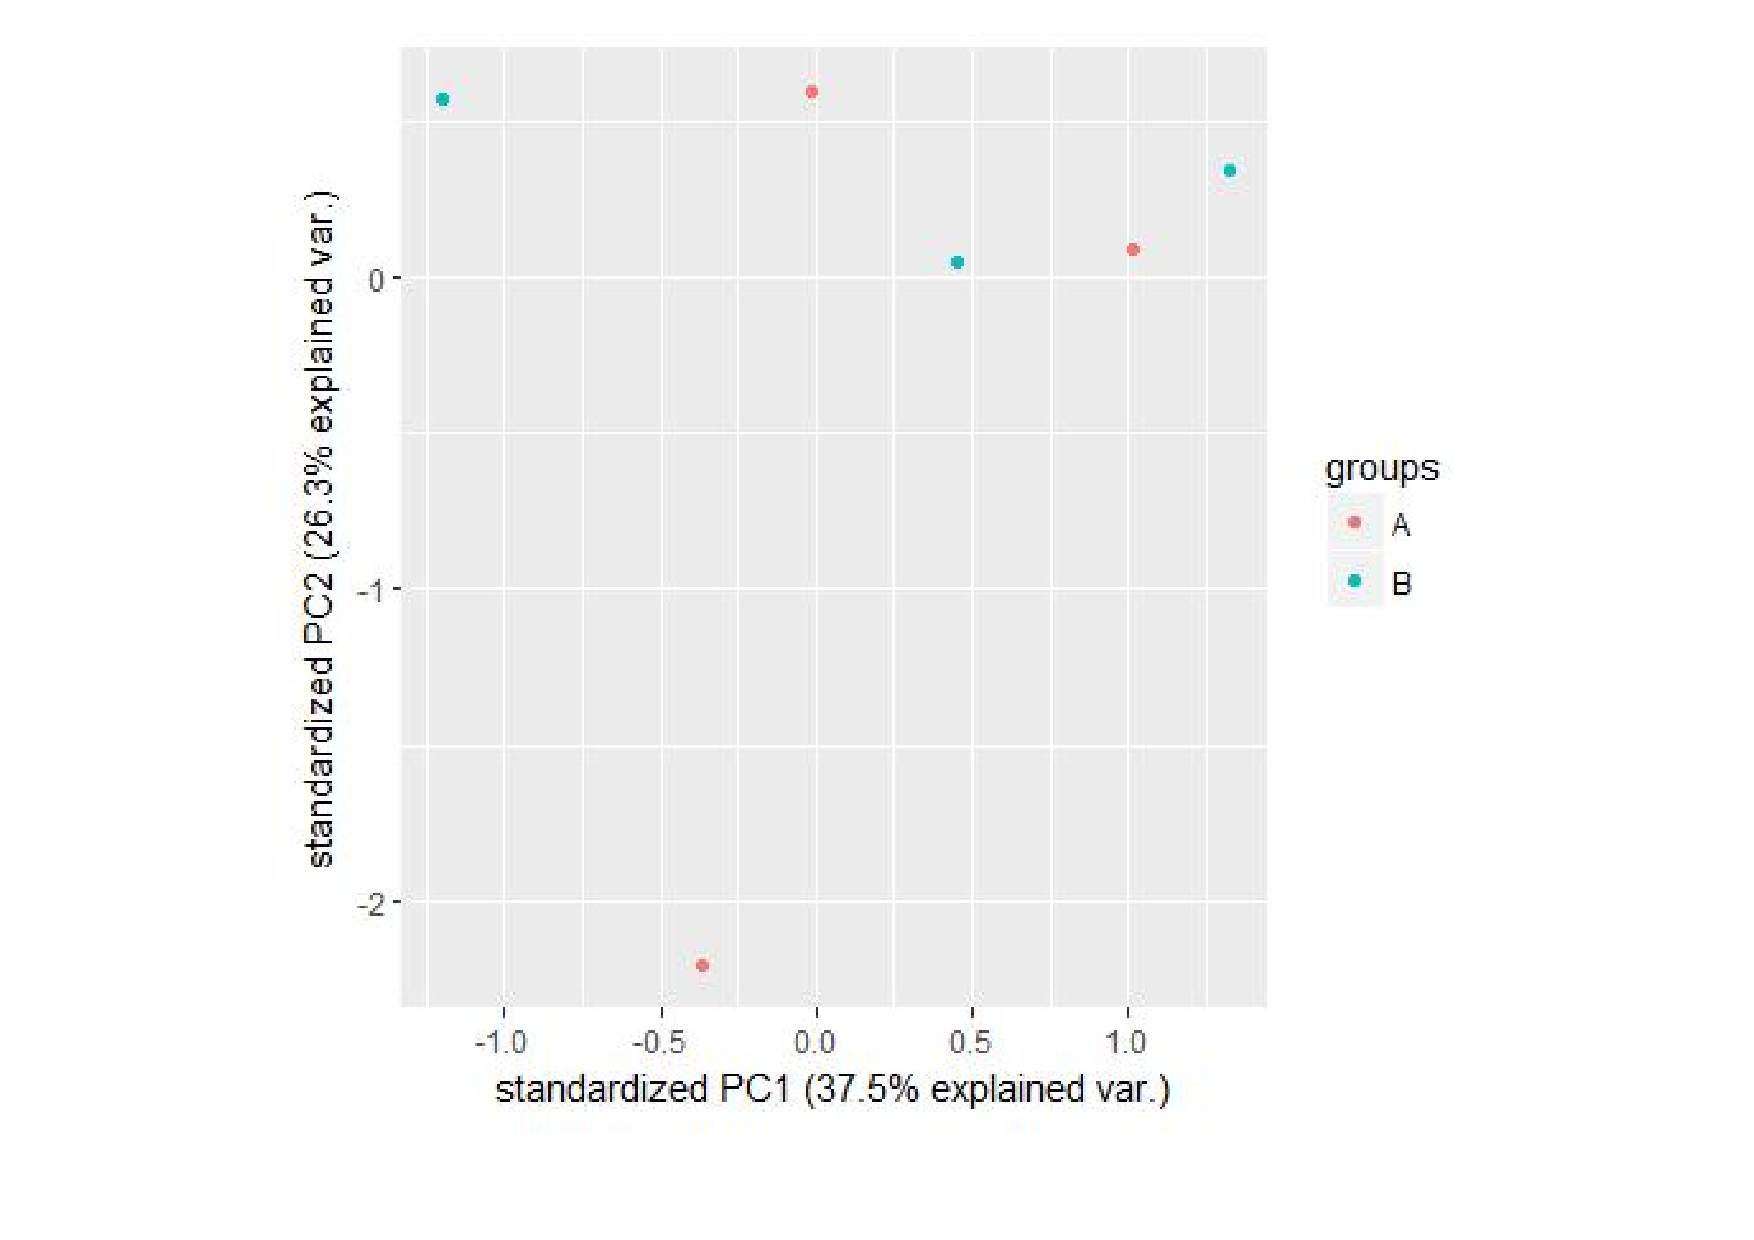
\includegraphics[width=5cm]{02.pdf}
\caption{word2vecによる分析結果}\label{分析結果}
\end{figure}

\section{考察}
図\ref{分析結果}では,一文章ごと結果がグラフにプロットされている.同段落内の文章は同じ話題でなければならないため,文章のベクトルも同じ方向性である必要がある.このことから,タグAの数値とタグBの数値がそれぞれ集中している事が必要であると仮定した.
しかし,本研究での分析結果は,同段落内の文章にもかかわらず,ベクトルは散らばって分布している事がわかることから,話題の方向性が違うと考えられるが,今回解析対象の文章は人間の添削を通し,文章に違和感や段落の方向性が同じと考えられるので,必ずしも本研究の解析結果が正しいとは限らないと考えることができる.

\section{結論}

今回の結果から,Word2vecを用いて数値によって文章を見ていくことで,個人の主観だけでなく,定量的に文章の書き方を定義できることも期待される.

\bibliographystyle{junsrt}
\bibliography{biblio}%「biblio.bib」というファイルが必要.

\end{document}
